
\label{sec:generalbackprop}

Backpropagation is a gradient-descent supervised learning algorithm 
in which the combination of weights that minimizes a given error function is considered to be a solution of the learning problem. It is suitable for both static and dynamic ANNs.

Generally speaking, a network represents a chain of function compositions which transform an input to an output vector. Each initialization of a network is a particular implementation
of that composite function. Thus, the learning problem consists of finding the optimal combination of weights so that the particular network function approximates a given function as closely as possible. However, the target function is a priori unknown; we only have some matching patterns.

As we explained in \subsecref{learningrules} when talking about supervised learning algorithms, the just mentioned patterns comprise our training set. Lets assume we are given a training set defined by $\{\mathbf{p_{1}} , \mathbf{t_{1}} \}, \{\mathbf{p_{2}} , \mathbf{t_{2}}\}, ...,
 \{\mathbf{p_{Q}} , \mathbf{t_{Q}} \}$
consisting of $Q$ ordered pairs of input $\mathbf{p}$ and target output $\mathbf{t}$ vectors.
At the beginning, 
when the input pattern $\mathbf{p}_{q}$ from the training set is presented to the neural network,
it produces an output vector $\mathbf{o}_{q}$ different in general from the target $\mathbf{t}_{q}$.
Hence, the final objective is to make $\mathbf{o}_{q}$ as equal as possible to $\mathbf{t}_{q}$ for $1 \leq q \leq Q$, which is possible by minimizing the error function of the network. 
The most common one chosen for backpropagation algorithms is the least mean squares
error-function defined as
\begin{equation}
E=\frac{1}{2}\sum_{q=1}^{Q}
\parallel \mathbf{t}_{q}-\mathbf{o}_{q} \parallel^2
\label{eq:globalerrorfunction}
\end{equation}

Since this minimization process requires the computation of the gradient of the error function at each iteration step,
we must guarantee the continuity and differentiability of the error function.
In view of the algorithm computes only function compositions, 
the foregoing is traduced in the usage of a kind of activation function that accomplished the characteristics of continuity and differentiability. 
Some examples of suitable activation functions are: 
the linear function, taking care in its variants to avoid the points where the derivative is undefined; 
the log-sigmoid and the hyperbolic tangent sigmoid functions. 
On the contrary, the hard-limit will be an instance of a non suitable function.

After minimizing the error function for the training set, 
new unknown input patterns are presented to the network. 
The expected behaviour of the network is being capable to interpolate; 
\ie, recognize whether the new input vector is similar to a learned pattern 
and, accordingly, produce the corresponding similar output.

The backpropagation algorithm is threfore used to find a local minimum of the error function. 
To do this, the network parameters are firstly initialized with a random function. 
Then, the gradient of the error function is recursively computed and
used to correct the initial weights.

Next sections explained the rules of the backpropagation algorithm as well as the necessary modifications for its usage in the different architectures of ANNs described in \secref{topologies}.

\subsection{Static backpropagation algorithm}
\label{subsec:staticbackprop}
The static backpropagation is suitable for feedforward neural networks such as those introduced in \subsecref{neuralnetworkmodel}. For an accurate explanation of the learning rules behind this training algorithm, lets imagine a multilayer network with one input layer, an indetermined number of hidden layers and one output layer.

In a given time, the connection between the neuron $j$ of the $l$-th layer and the neuron $i$ of the $(l-1)$-th layer has a weight value of $w_{ji}$. The output $a$ of neuron $j$ for the input pattern $\mathbf{p}_{q}$ can be expressed in terms of the net input $n$ and the connection weights as follows
\begin{equation}
a_{qj}=f_{j}(n_{qj})=f_{j}(\sum_{i\in \Gamma_{j}}w_{ji}a_{qi})
\label{eq:neuronjoutput}
\end{equation}
where $\Gamma_{j}$ denotes the set of presynaptic neurons of the postsynaptic neuron $j$.

What is really intended is to compute the gradient of the error function. 
Since the weights are the parameters we can modify in order to produce the correct network output, 
this gradient is defined by the partial derivative with respect to the weights of the connections between the corresponding neurons. Hence, for each pattern $q$, the gradient of the error function evaluated in neuron $j$ is
\begin{equation}
\frac{\partial E_{q}}{\partial w_{qji}}
\label{eq:gradienterrorfunction}
\end{equation}

With \eref{neuronjoutput} and making use of the chain rule, Expression \ref{eq:gradienterrorfunction} can be transformed into
\begin{equation}
\frac{\partial E_{q}}{\partial w_{qji}}=
\frac{\partial E_{q}}{\partial n_{qj}}
\frac{\partial n_{qj}}{\partial w_{qji}}=
\frac{\partial E_{q}}{\partial n_{qj}} a_{qj}=
-\delta_{qj} a_{qj}
\label{eq:chainrulegradienterrorfunction}
\end{equation}
where $\delta_{qj}$ is a variable introduced just for a matter of notation.

Analising the sign of the above equation, two cases can be distinguished:
\begin{itemize}

\item If $\delta_{qj}a_{qj}<0$, the gradient of the error function is positive, which means that $E_{q}$ increases (decreases) when $w_{ji}$ rises (falls). In view of this, for getting a lower value of $E_{q}$ we only have to reduce the value of $w_{ji}$ in a controled way. The manner in which backpropagation update the weight value is by adding it the negative amount of $\delta_{qj}a_{qj}$ (remember that $\delta_{qj}a_{qj}<0$ in this case) multiplied by the constant $\mu$. This latter parameter is known as the \emph{learning rate of the algorithm} and it controls how big/small is the amount added to $w_{ji}$. 

\item The same reasoning is applied whether $\delta_{qj}a_{qj}>0$. In this case, $E_{q}$ decreases when $w_{ji}$ rises. The updated value of $w_{ji}$ can be therefore obtained by adding it the positive amount of $\delta_{qj}a_{qj}$ multiplied again by $\mu$.

\end{itemize}

Thus, the updating condition of each weight $w_{ji}$ can be expressed mathematically as
\begin{equation}
w_{ji}\leftarrow w_{ji}+ \mu\delta_{qj}a_{qj}
\Leftrightarrow 
\Delta w_{ji}= -\mu\delta_{qj}a_{qj}
\label{eq:updatingrule}
\end{equation}

The remainder is know how obtain the $\delta_{qj}$. Using the chain rule again and the first part of \eref{neuronjoutput}, we can expressed the mentioned term as
\begin{equation}
\delta_{qj}= 
- \frac{\partial E_{q}}{\partial n_{qj}}=
- \frac{\partial E_{q}}{\partial a_{qj}}
\frac{\partial a_{q}}{\partial n_{qj}}
\label{eq:factordelta}
\end{equation}

Since $a_{j}=f_{j}(n_{j})$, then
\begin{equation}
\frac{\partial a_{q}}{\partial n_{qj}}=
f_{j}'(n_{j})
\label{eq:factoractivationfunction}
\end{equation}
and only the first factor of the right part of \eref{factordelta} lasts. 

For its calculation, it is necessary to distinguished two situations:
\begin{itemize} 
\item If $j$ is an output-layer neuron, assuming that the output space is S-dimensional (\ie, $\in\mathbb{R}^S$), the output layer of the feedforward NN will be comprised by S neurons. Thus, \eref{globalerrorfunction} can be rewritten, for each pair $q$ of target-output vectors, as 
\begin{equation}
E_{q}=\frac{1}{2}\sum_{j=1}^{S} (t_{qj}-o_{qj})^2
\label{eq:patternerrorfunction}
\end{equation}

This way, and knowing that in this case $a_{j}=o_{qj}$ where $o$ denotes the output of the whole network, it is accomplished that
\begin{equation}
-\frac{\partial E_{q}}{\partial a_{qj}} =
-\frac{1}{2}\frac{\partial o_{qj}}{\partial}
\sum_{j=1}^{S} (t_{qj}-o_{qj})^2 =
...= t_{qj}-o_{qj}
\label{eq:factortarout}
\end{equation}

Finally, combining Equations \ref{eq:factordelta}, \ref{eq:factoractivationfunction} and \ref{eq:factortarout} we obtain
\begin{equation}
\delta_{qj}= f_{j}'(n_{j})(t_{qj}-o_{qj})
\label{eq:deltajoutput}
\end{equation}


\item If $j$ is not an ouput-layer neuron, then there will be a neuron $k$ in the $(l+1)$-th layer with a net input $n_{qk}$ when the pattern $q$ is presented to the network. Hence,
\begin{equation}
\frac{\partial E_{q}}{\partial a_{qj}}=
\sum_{j\in \Gamma_{k}}
\frac{\partial E_{q}}{\partial n_{qk}}
\frac{\partial n_{qk}}{\partial a_{qj}}=
\sum_{j\in \Gamma_{k}}
\frac{\partial E_{q}}{\partial n_{qk}}
\frac{\partial}{\partial a_{pj}}
\sum_{i\in \Gamma_{j}}w_{ji}a_{qi}= 
-\sum_{j\in \Gamma_{k}}\delta_{qk}w_{ji}
\label{eq:factorbackpropagated}
\end{equation}

Finally, combining Equations \ref{eq:factordelta}, \ref{eq:factoractivationfunction} and \ref{eq:factorbackpropagated} we obtain
\begin{equation}
\delta_{qj}= f_{j}'(n_{j})
\sum_{j\in \Gamma_{k}}\delta_{qk}w_{ji}
\label{eq:deltajNOoutput}
\end{equation}

\end{itemize}

The idea of the backpropagation algorithm is to update recursively each weight term.
Therefore, the steps to follow and repeat until the error function reaches a minimum are:
\begin{enumerate}
\item Present an input pattern $\mathbf{p}_{q}$ and calculate the error function with the network output $\mathbf{o}_{q}$ and the target $\mathbf{t}_{q}$ vectors with \eref{patternerrorfunction}.
\item Obtain the output $a_{qj}$ of each neuron $j$ of the network making use of \eref{neuronjoutput}.
\item Update each weight term with the rule of \eref{updatingrule}, where the $\delta_{qj}$ term follows \eref{deltajoutput} in case of an output-layer neuron and \eref{deltajNOoutput} it is a hidden-layer neuron.
\end{enumerate}


\subsubsection{Convergence}
\label{subsubsec:backpropconvergence}
???????????


\subsection{Backpropagation through time}
\label{subsec:bptt}
Backpropagation through time (BPTT) is a variant of the above backpropagation algorithm. While the latter is used to train static feedforward networks, the BPTT is suitable for recurrent neural networks.

BPTT algorithm begins by unfolding the dynamic network into a multilayer feedforward one. The new topology has a layer for each time step in the sequence, as if the time step is the index of the layer. During this process, the connections between layers mus be redirected too. Then, the static backpropagation algorithm can be used for training the feedforward network obtained. 
\figref{bpttunfolding} shows how the unfolding process of depth $3$ (three time steps) is carried out.

\begin{figure}[!ht]
\centering
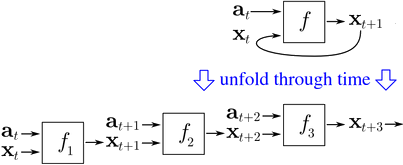
\includegraphics[width=0.6\textwidth]{images/unfoldOverTime.png}
\caption{A recurrent network unfolding process}
\label{fig:bpttunfolding}
\end{figure}

Notice that, since layers have been obtained by replicating the recurrent network over and over,
 weights in all layers should be the same.
Thus, BPTT updates all equivalent weights using the sum of the gradients obtained for weights in all layers.

In practice, this alogithm has an important drawback: 
the entire time series must be used, 
so its application becomes hard if online adaptation is required. 
In order to avoid this situation, 
a possibility is to truncate the time series. However, the memory beyond truncated time 
cannot be captured by the model.

\subsection{Backpropagation for spiking neural networks}

\label{subsec:snnbackprop}
As we described in \subsecref{ANN:SNN}, SNN incorporate spatial-temporal information. Therefore, the new backpropagation algorithm must do the same. The following lines try to describe how the already-known learning rules are adapted to a SNN where each neuron is not limited to spike only once.
More details of the process can be found in \cite{booij2005gradient}.

Firstly, taking into account that the inputs and outputs of a SNN are firing times, the error function for each pattern described in \eref{patternerrorfunction} is adapted as follows:
\begin{equation}
E=\frac{1}{2}\sum_{j=1}^{S} (t_{j}^{d}-t_{j}^{a})^2
\label{eq:patternerrorfunctionSNN}
\end{equation}
where $j$ denotes each neuron of the $S$-dimensional output-layer, and $\{t_{j}^{d}\}=\mathcal{F}_{j}^{d}$ and $\{t_{j}^{a}\}=\mathcal{F}_{j}^{a}$ represent the set of desired spike times and actual firing times respectively.

For error-backpropagation, we treat each one of the $1 \leq k \leq m$ synaptic terminals as a separate connection. Hence, for the 
updating rule in \eref{updatingrule} using the gradient descent method, we need to calculate:
\begin{equation}
\Delta w_{ji}^{k}= -\mu\frac{\partial E}{\partial w_{ji}^{k}}
\label{eq:updatingruleSNN}
\end{equation}
where $\mu$ is the learning rate and $w_{ji}^{k}$ denotes the weight of the $k$-th connection between the presynaptic neuron $i$ and the postsynaptic neuron $j$. 
Other parameters in SNN like the axonal delays $d_{ji}^{k}$ have also be tuned to reduce the error function \cite{schrauwen2004extending}.


As it is expressed in \eref{thresspikecondition},
the time when a spiking neuron $j$ fires is function of the membrane potential $u_{j}(t)$, which depends in turn on the weights $w_{ji}^{k}$ as formulated in \eref{srmmultipleconnections}. Besides, because neurons can fire multiple times, the above equation must be expanded to
\begin{equation}
\Delta w_{ji}^{k}= -\mu
\sum_{f\in \mathcal{F}_{j}}
\frac{\partial E}{\partial t_{j}^{(f)}}
\frac{\partial t_{j}^{(f)}}{\partial w_{ji}^{k}}
\label{eq:updatingruleSNNmultiplespikes}
\end{equation}
where $\mathcal{F}_{j}$ denotes the spike train of each neuron $j$. This way, the updated weight is assigned to the subsequent spike at the time of its arrival at the synapse.

The derivative of the firing time with respect to the weight can be computed starting out with the thresholding condition of $u_{j}(t)$, in which $u_{j}(t_{j})=\vartheta$. The resultant expression is (see \cite{bohte2002error} and \cite{booij2004temporal} for a complete derivation)
\begin{equation}
\frac{\partial t_{j}^{(f)}}{\partial w_{ji}^{k}}
=
\frac{\partial u_{j}(t_{j}^{(f)})}{\partial w_{ji}^{k}}
\frac{-1}{\frac{\partial u_{j}(t_{j}^{(f)})}{\partial t_{j}^{(f)}}}
\label{eq:dtdw}
\end{equation}

We can derive the partial derivative of the potential during a spike $t_{j}^{(f)}$ with respect to the weight from \eref{srmmultipleconnections}.
We must keep in mind that earlier spikes $t_{j}^{(e)}<t_{j}^{f}$ also depend on the same weight and influence the potential, so the function becomes recursive
\begin{equation}
\frac{\partial u_{j}(t_{j}^{(f)})}{\partial w_{ji}^{k}}
=
-\sum_{e\in \mathcal{F}_{j}}\eta'(t_{j}^{(f)}-t_{j}^{(e)})
\frac{\partial t_{j}^{(e)}}{\partial w_{ji}^{k}}
+
\sum_{l\in \mathcal{F}_{i}}\varepsilon(t_{j}^{(f)}-t_{i}^{(l)}-d_{ji}^k)
\label{eq:dudw}
\end{equation}

It is worth highlighting that it is not explicitly required that $t_{j}^{(e)}<t_{j}^{(f)}$ beacuse this condition is already met due to the fact that $\eta(t)=\varepsilon(t)=0~\text{for}~t\leq 0$.

The denominator of the second factor of \eref{dtdw} can be calculated as
\begin{equation}
\frac{\partial u_{j}(t_{j}^{(f)})}{\partial t_{j}^{(f)}}
=
\sum_{e\in \mathcal{F}_{j}}\eta'(t_{j}^{(f)}-t_{j}^{(e)})
+
\sum_{i\in \Gamma_{j}}
\sum_{l\in \mathcal{F}_{i}}
\sum_{k=1}^{m}
	w_{ji}^{k}\varepsilon'(t_{j}^{(f)}-t_{i}^{(l)}-d_{ji}^k)
\label{eq:dudt}
\end{equation}

Once we can compute the entire expression of \eref{dtdw}, we calculate the first derivative factor of \eref{updatingruleSNNmultiplespikes}. 
Its expression is derived for every spike of non-output neuron, 
which depends on all spikes produced by all its postsynaptic neurons $h$:
\begin{equation}
\frac{\partial E}{\partial t_{j}^{(f)}}
=
\sum_{h\in \Gamma{j}}
\sum_{g\in \mathcal{F}_{h}}
\frac{\partial E}{\partial t_{h}^{(g)}}
\frac{\partial t_{h}^{(g)}}{\partial t_{j}^{(f)}}
\end{equation}
where the derivative of a postsynaptic spike $t_{h}^{(g)}$ with respect to a presynaptic $t_{j}^{(f)}$ spike can be further expanded as in equation \eref{dtdw}:
\begin{equation}
\frac{\partial t_{h}^{(g)}}{\partial t_{j}^{(g)}}
=
\frac{\partial u_{h}(t_{h}^{(g)})}{\partial t_{j}^{(f)}}
\frac{-1}{\frac{
\partial u_{h}(t_{h}^{(g)})}{\partial t_{h}^{(g)}}}
\end{equation}

The second factor is calculated with \eref{dudt}; the derivative of the potential during a postsynaptic spike with respect to a presynaptic spike, can again be derived from \eref{srmmultipleconnections} as follows
\begin{equation}
\frac{\partial u_{h}(t_{h}^{(g)})}{\partial t_{j}^{(f)}}
=
-\sum_{n\in \mathcal{F}_{j}}\eta'(t_{h}^{(g)}-t_{h}^{(n)})
\frac{\partial t_{h}^{(n)}}{\partial t_{j}^{(f)}}
-
\sum_{k=1}{m}w_{hj}^{k}\varepsilon'(t_{h}^{(g)}-t_{j}^{(f)}-d_{hj}^k)
\end{equation}

Notice that all are recursive functions, 
which is the temporal equivalent of the conventional backpropagation technique,
where the error was back-propagated spatially through the network. The order in which the calculations are done is therefore paramount.

